\label{sec:2norm}
%Often ad hoc rules based on size of preview gains (ref), or area under graph of preview gains....
The purpose of this section is to derive an efficient means of computing the minimum achievable closed-loop $\htwo$ norm for a given preview length. In so doing we provide tools to answer the questions: 
\begin{itemize}
\item What is the preview length required to achieve a given performance specification?
\item What is the maximum possible reduction in the closed-loop $\htwo$-norm through preview?
\item If a large amount of preview is available, how much should be used?
\end{itemize}


\begin{figure}
\begin{center}
\stdcontrolfrags
\psfrag{Khat}{$\hat K$}
\psfrag{Ghat}{$\hat G$}
\psfrag{rhat}{$\hat r$}
\scalebox{0.8}{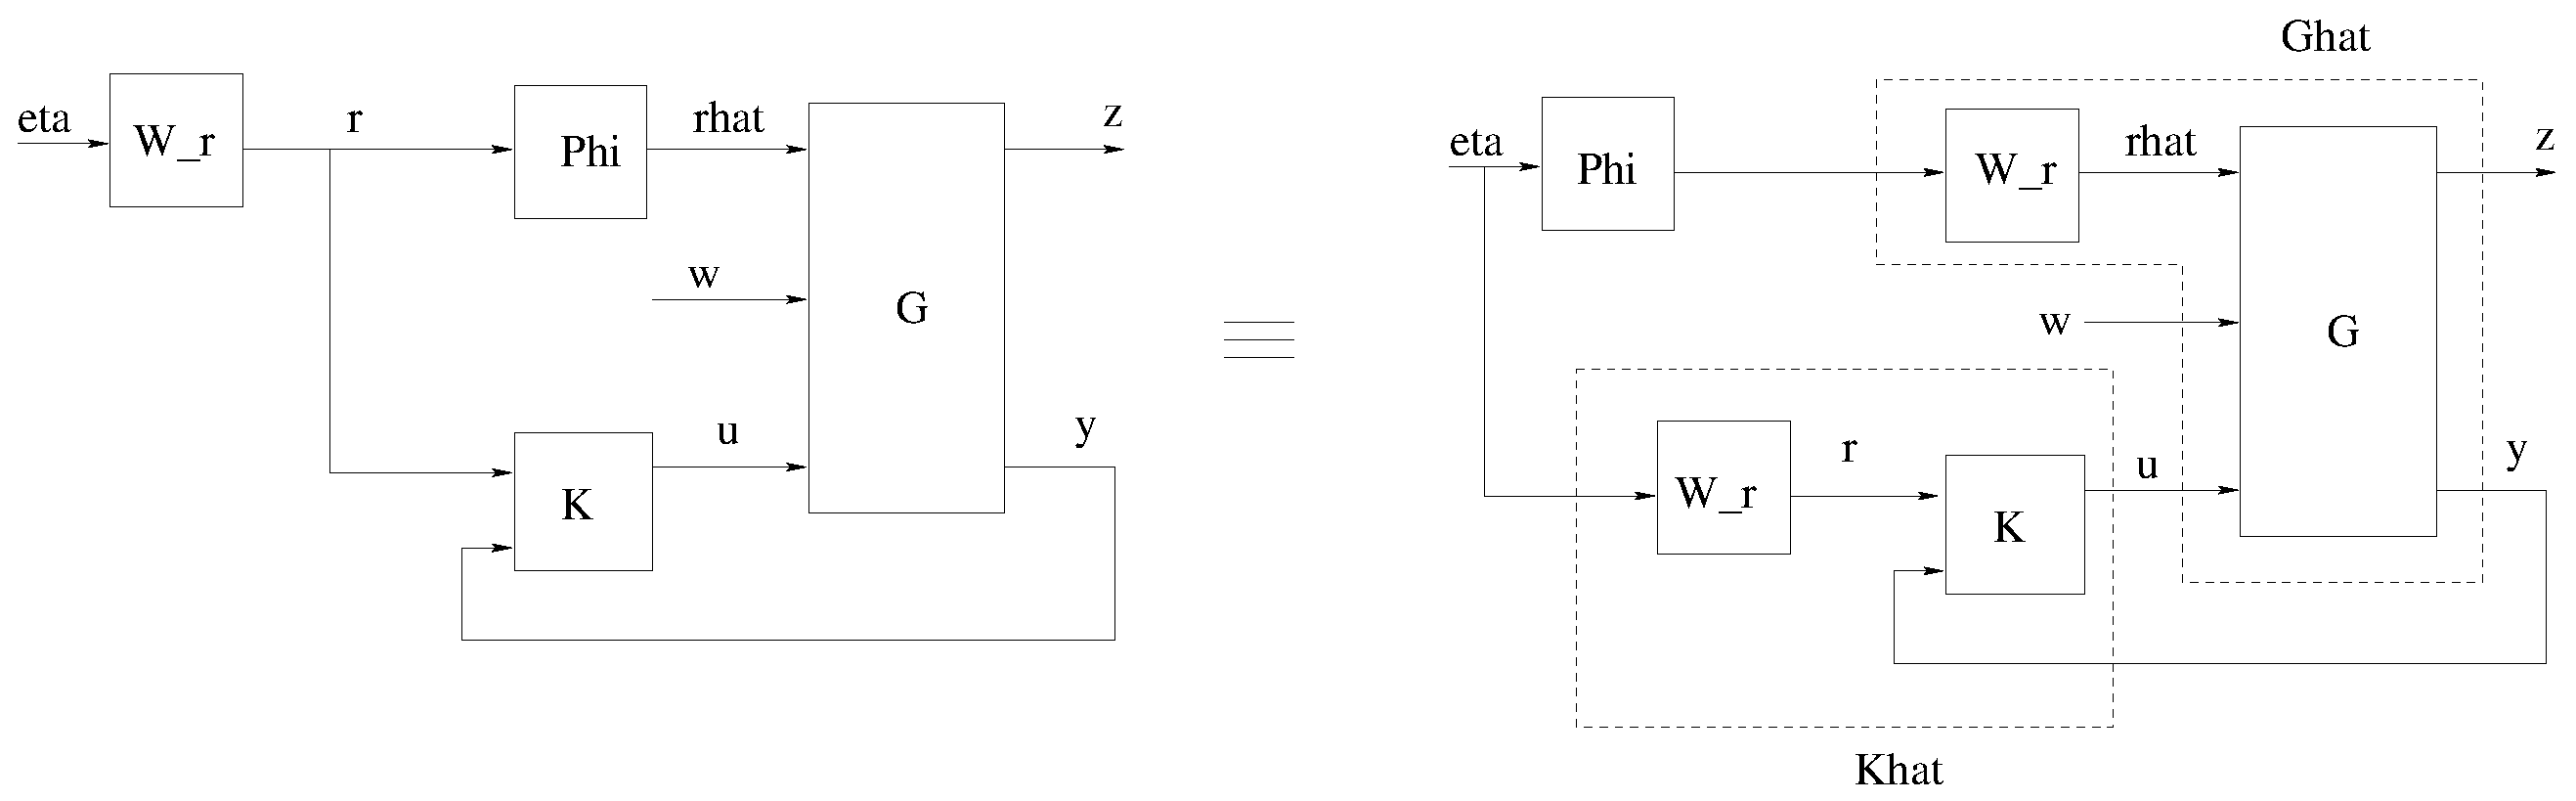
\includegraphics[width=1.4\columnwidth]{./diags/DistRejSysEquiv.eps}}
\end{center}
\caption{Two equivalent representations of the previewable disturbance rejection problem. These representations are equivalent in the sense that the transfer functions from $\eta$ and $w$ to $z$ and $y$ are identical. Recall that $\Phi=\z^{-N}I$, which commutes with $W_r$ under multiplication. \label{fig:AbsorbWr}}
\end{figure}

For the purposes of computing the minimum achievable $\htwo$-norm, we may assume $W_r=I$ without loss of generality. The transformation that enables us to make this assumption is illustrated in Figure~\ref{fig:AbsorbWr}. The design problem involving $\hat K$ and $\hat G$ is clearly a problem of the class of Figure \ref{fig:DistRejSys}, but without a pre-filter. The achievable $\htwo$-norm will be the same in either case, and in this section we will work with the simpler problem setup, where it is assumed that $W_r$ has been absorbed into $\hat G$ and $\hat K$. This transformation is not used in the preceding sections because it obscures the impact of $W_r$ on the control signal, and because we would be required to perform further manipulations in order to remove the additional controller states resulting from the extra copy of $W_r$. 

It is easy to check that the results of the previous sections carry over for $W_r=I$. All that is required is to remove the  gains associated with the states of $W_r$.

We note again that:
% 
\begin{equation}
\nrm{T_{{[r'\,\,w']'}\rightarrow z}}^2_2 =
\nrm{T_{w\rightarrow z}}^2_2+
\nrm{T_{r\rightarrow z}}^2_2. \label{proj_prop}
\end{equation}
%
As observed in Corollary~\ref{cor:minwandr}, the optimal preview controller minimises $\nrm{T_{w\rightarrow z}}_2$. Since $X_{gg}$ and $Y_g$ are the solutions to the DAREs associated with the problem of minimising $\nrm{T_{w\rightarrow z}}_2$, we may use the results in Sections \ref{subsec:stdH2FI} and \ref{subsec:stdH2OF} to write:
\als{
\gamma_{wc}^2&=\textrm{Tr}\left\{(D_{11gw}+D_{12}F_{0w})'(D_{11gw}+D_{12}F_{0w})\right.\\ &\left.\qquad+(B_{1gw}+B_{2g}F_{0w})'X_{gg}(B_{1gw}+B_{2g}F_{0w})\right\}\\
\gamma_{wf}^2&=\textrm{Tr}\left\{\bar R\left( (L_{0y}D_{21gw}-F_{0w})(L_{0y}D_{21gw}-F_{0w})'\right.\right.\\ &\left.\left.\qquad+(L_{0y}C_{2g}-F_{2g})Y_{gg}(L_{0y}C_{2g}-F_{2g})'\right) \right\}\\
\nrm{T_{w\rightarrow z}}^2_2&=\gamma_{wc}^2+\gamma_{wf}^2,
} 
which are independent of the preview length.

We now turn our attention to the evaluation of $\nrm{T_{r\rightarrow z}}_2$. Since the signal $r$ is `known' to the controller, it does not introduce an estimation error. As a result the output feedback controller achieves exactly the same transfer function $T_{r\rightarrow z}$ as the full-information controller, $K_{FI}$. Thus:
\als{
T_{r\rightarrow z}=\ssmodf{A+B_2F_2}{\ma{B_{2g}F_{0r}\\B_p}}{C_1+D_{12}F_2}{D_{12}F_{0r}}.
}
%
Note that $X$ satisfies: 
\als{(A+B_2F_2)'X(A+B_2F_2)+(C_1+D_{12}F_2)'(C_1+D_{12}F_2),}
and so using equation (\ref{eqn:2normcomp}) we may write:
\als{
\nrm{T_{r\rightarrow z}}^2_2 &=\tra{\left(D_{12}F_{0r}\right)'D_{12}F_{0r}+\ma{B_{2g}F_{0r}\\B_p}'\ma{X_{gg}&X_{gp}\\X_{gp}'&X_{pp}}\ma{B_{2g}F_{0r}\\B_p}}.
} 
\mbox{where $F_{0r}=-{\bar R}^{-1}B_{2g}'X_{gp}B_p$. The above expression may be simplified to} 
\aln{
\nrm{T_{r\rightarrow z}}^2_2&=\tra{B_p'X_{pp}B_p-F_{0r}'\bar RF_{0r}\label{eqn:gamrmedeff}}.
}
%
Our next task is to find an efficient method for computing $B_p'X_{pp}B_p$. Using the $W_r=I$ version of (\ref{eqn:Xdd}), we can write:
\als{
X_{pp}&=A_p'X_{pp}A_p+\hat Q-F_{2p}'\bar{R}F_{2p}\\
\mbox{in which} \\
\hat Q &= C_{p}'B_{1gr}'X_{gg}B_{1gr}C_{p}+A_p'X_{gp}'B_{1gr}C_{p}+C_{p}'B_{1gr}'X_{gp}A_p+C_{p}'D_{11gr}'D_{11gr}C_{p}.
}

Substituting this into itself leads to:

\als{
X_{pp}=\sum^{N-1}_{j=0}{A_p^j}'(\hat Q - F_{2p}'\bar{R}F_{2p})A_p^j.
}
%
Note that post-multiplying by $A_p^kB_p$ has the effect of selecting individual block columns of the preceding matrix, that $C_pA_p^kB_p=0 \,\, \forall k \neq N-1$, and that $A_p^N=0$. This means that:
%
\[
B_p'X_{pp}B_p=B_{1gr}'X_{gg}B_{1gr}+D_{11gr}'D_{11gr}-F_{2p0}'\bar{R}F_{2p0} - \sum_{j=0}^{N-2}S' A^j_{cg} B_{2g} {\bar R}^{-1} B_{2g}' {A^j_{cg}}' S,
\]
where $F_{2p0}$ is the left-most block column of $F_{2p}$ and is given by:
\begin{equation}
F_{2p0}=-\bar R^{-1}\left(B_{2g}'X_{gg}B_{1gr}+D_{12}'D_{11gr}\right). \label{eqn:F2p0}
\end{equation}
%
Combining this with (\ref{eqn:gamrmedeff}), and using (\ref{eqn:Xgp}), leads to 
\aln{
\nrm{T_{r\rightarrow z}}^2_2=\tra{\underbrace{B_{1gr}'X_{gg}B_{1gr}+D_{11gr}'D_{11gr}-F_{2p0}'\bar{R}F_{2p0}}_{\mbox{Zero preview}}-\underbrace{\sum_{j=0}^{N-1}S' A^j_{cg} B_{2g}{\bar R}^{-1} B_{2g}'{A^j_{cg}}'S}_{\mbox{Preview reduction}}}.
\label{eqn:H2CostSplit}}
In order to judge how much preview to use, we need to know the value of the maximum possible improvement due to preview action. Suppose the matrix $\Gamma$ satisfies:
\als{
\Gamma=A_{cg}\Gamma A_{cg}'+B_{2g}\bar R^{-1}B_{2g}'
,}
which implies that:
\als{
\Gamma=\sum_{j=0}^{\infty}A_{cg}^jB_{2g}\bar R ^{-1}B_{2g}'{A_{cg}'}^{j}
.}
Comparing this to (\ref{eqn:H2CostSplit}), it follows that the reduction in $\nrm{T_{r\rightarrow z}}_2^2$ due to preview is bounded above by 
\[
\tra{S'\Gamma S},
\]
and evaluating this limit only requires the solution of an $n_g$-dimensional Lyapunov equation (in addition to the $n_g$ dimensional DARE required to evaluate $S$). The following quantity provides a useful measure of the fraction of the maximum norm reduction that has been achieved:
\aln{\gamma_{\,_{\%,imp}}=100\times \tra{S'\Gamma S}^{-1}{\left(\sum_{j=0}^{N-1}S' A^j_{cg} B_{2g}{\bar R}^{-1} B_{2g}'{A^j_{cg}}'S\right)}.\label{eqn:gamimp}} 
%This provides a useful bound on the achievable norm reduction one might obtain using preview. 
This can be used to determine how much preview to use; for example, one might continue adding preview points until $\gamma_{\,_{\%,imp}} >99\%$.
